% !TeX root = ../main.tex

\chapter{绪论}

\section{引言}

自上世纪以来,实现人工智能 (Artificial Intelligence, AI) 是许多学者的梦想。在许多来自不同领域的学者们的共同不懈地努力下,人工智能至今已经取得了长足的发展。当下,人工智能已经能够完成多样复杂的任务,如识别复杂物体\cite{he2016deep}、识别语音内容\cite{luong2015effective}、处理自然语言\cite{amodei2016end}、过滤社交网络信息、机器翻译\cite{bahdanau2014neural}、设计药物、分析医疗图像\cite{esteva2017dermatologist}和材料审查等任务。因此,人工智能被广泛地用于人类社会中的各个领域中,以帮助人类更快的解决完成处理信息问题。但纵观人工智能的发展历史,其并不是一路向上,而是经历了60年的沉浮,并且其深刻地受到了计算机硬件技术发展的影响。总的来说,如图\ref{devlop}所示人工智能的发展经历了三次高峰。

\begin{figure}[ht]
	\centering
	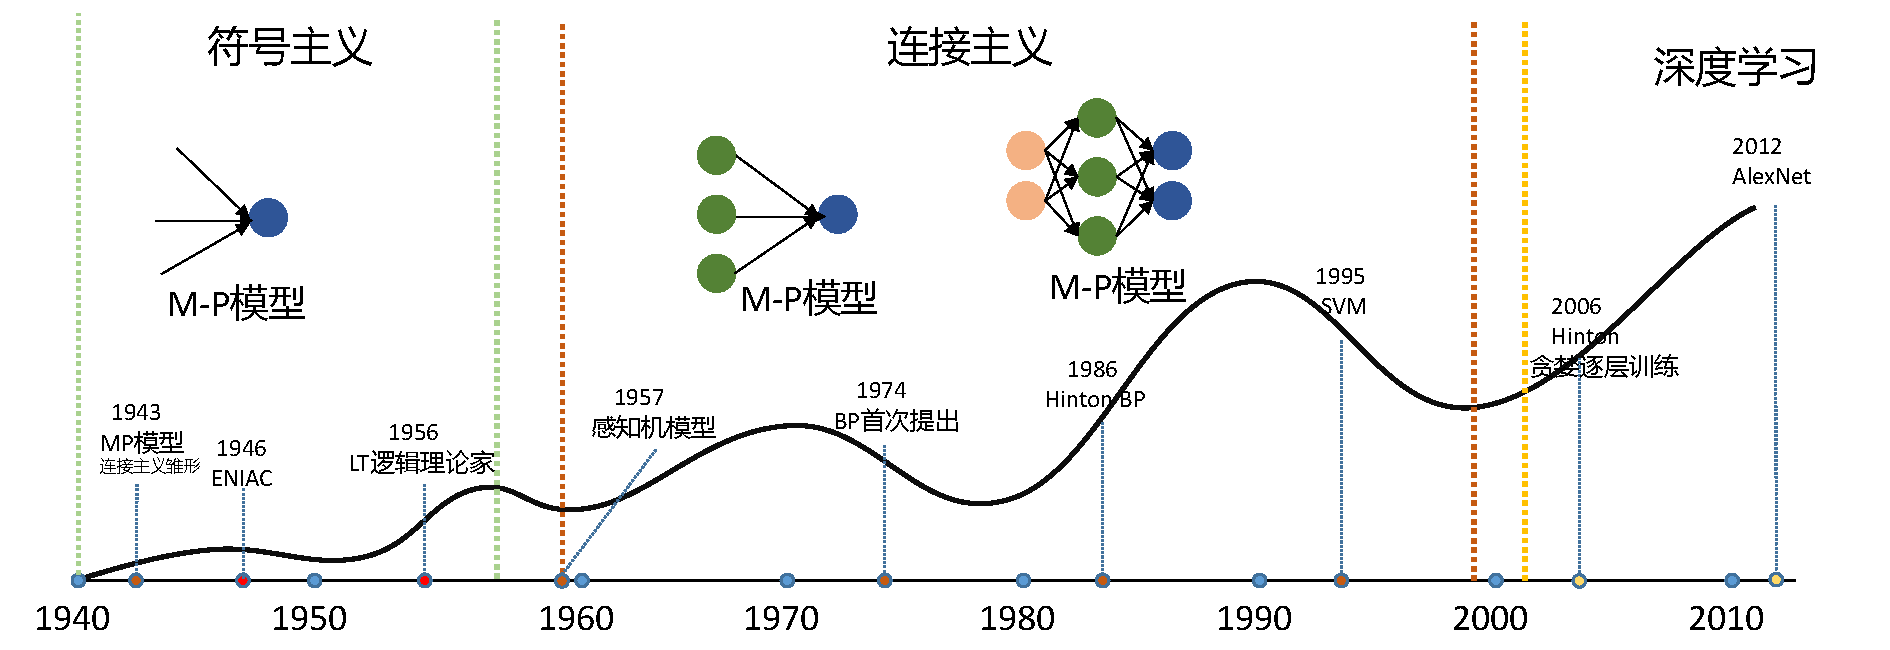
\includegraphics[width=1\textwidth]{figures/development.pdf}
	\caption{人工智能发展历史}
	\label{devlop}
\end{figure}

人工智能的第一次高峰是20世纪40年代-60年代的控制论。彼时的学者认为人工智能起源于数理逻辑,希望用数理逻辑描述生物智能行为。符号主义是纯数学上的逻辑推理的,即将输入数据转换成逻辑表达,用符号演算的形式化方法进行逻辑推理,尚无训练的概念。1956年Simon开发出一个启发程序“LT逻辑理论家”,能够证明38条数学定理。随后符号主义学派发展了启发式算法、专家系统、知识工程理论等。但符号主义学派框架下的人工智能需要足够多的先验知识,人工智能并不具备自主学习的能力,这一缺陷使得人工智能只能处理相对简单的任务。此后符号主义发展缓慢,人工智能进入瓶颈期。人工智能的第二次高峰是20世纪80年代-90年代的连接主义。自1946年第一台通用计算机ENIAC诞生和随后几十年计算机算力的飞速发展,人工智能的研究思路从数理逻辑的符号主义,逐步切换到连结主义和概率统计模型的新方法。连接主义认为人工智能起源于仿生学,其首次诞生于1943年,神经生理学家Warren McCulloch和数学家Walter Pitts对生物神经元建模,提出了一种神经元M-P模型。在M-P模型基础之上,1957年Frank Rosenblatt将多个M-P模型组合叠加,提出了感知机模型 (Perceptron)。受限于彼时计算机算力的不足,Frank Rosenblatt在1960年用硬件电路实现了第一个神经网络。随后,Paul Werbos在1974年提出了反向传播算法 (Backpropagation) 成功的让感知机具备了学习线性不可分函数的能力。人工智能进入到一个高速发展的黄金时期。但在20世纪90年代中期,Vapnik等人提出了比神经网络更高效,无须调参,泛化性能优异的支持向量机 (SVM),它同样可以解决线性不可分的问题,支持向量机的出现迅速打败了神经网络。同时,受限于当时计算机算力的制约和数据量,人工智能未能走出实验室进行大规模的应用。人工智能的第三次高峰是2006年至今的深度学习。2006年,Hinton提出贪婪逐层的训练方法,这个技术能够有效训练深度神经网络,但彼时的算力并不支持该技术的实施。后在2012年,Alex等人借助于分布式GPU的计算能力,成功训练出深度神经网络AlexNet斩获Imagenet比赛冠军。同时,各类移动计算设备的计算能力也快速提升。2017年苹果发布第一款人工智能芯片A11,该芯片首次搭载了神经网络引擎处理单元 (NPU)。此后人工智能开始飞速发展,硬件算力的提升加上多种新方法的涌现,人工智能走向市场,并被广泛地应用于无人驾驶、无人机、智能手机、智能眼镜、机器人等应用。


在所有深度学习方法中,卷积神经网络 (Convolutional Neural Networks, CNN) 以其优异的性能受到了大量学者的广泛关注。卷积神经网络是一类以卷积运算为主、有较深层次结构、具有表征学习能力 (representation learning)的前馈神经网络。卷积神经网络的首次提出是在1998年,Yann LeCun等人提出一个小型卷积网络LeNet,用于手写字符识别任务\cite{lecun1998gradient}。该项工作首次定义了CNN网络的结构的基本框架:卷积层+池化层+全连接层。随后,在2012年举办的大规模图像识别竞赛 (ImageNet Large Scale Visual Recognition Challenge,ILSVRC)中,Krizhevsky 等人提出的深度卷积神经网络AlexNet\cite{krizhevsky2012imagenet}以超过第二名10.9个百分点的识别准确度斩获ImageNet比赛的冠军。该工作有力地证明了卷积神经网络的学习能力。此后,随着GPU算力的不断提升,卷积神经网络的层数也不断加深。如2014年提出的有19层深度的 VGGNet\cite{simonyan2014very}和2015年提出的有22层深度的GoogLeNet\cite{szegedy2015going}。在以往的研究工作中,学者们普遍认为卷积神经网络的拟合能力由模型层数决定,即模型层数越多,网络的拟合能力越强。但事实上,随着网络层数的增多,卷积神经网络会出现退化问题 (Degrade Problem),即卷积神经网络层数到达一定深度后,拟合能力会出现退化,在测试集上的误差反倒会上升。2015年的ResNet\cite{he2016deep}提出使用跳层连接(shortcut)来减少梯度消失的问题。该工作成功的解决了神经网络层数增多后出现的拟合能力退化的问题,并首次将神经网络层数增加到了152层,并将imagnet数据集上识别准确率提高到96.5\%。同时,在其他各个领域学者们的合力推动下,卷积神经网络在目标检测、语义分割、人脸识别等其他计算机视觉任务也取得了巨大的成功。

目前,随着各类移动计算设备的算力和存储空间的飞速提升,卷积神经网络已成为许多智能化系统中的基本工具。但现有的卷积神经网络模型需求的计算资源和硬件实际能提供的计算资源供需之间仍然存在不匹配:1)神经网络模型尺寸远远大于计算设备可提供DRAM空间;2)神经网络模型的计算量远远大于计算设备可提供的计算资源。其中,第一个挑战决定了是否可以将神经网络部署在移动计算设备上进行处理。第二个挑战则决定了神经网络是否可以满足某些特定实时场景下的推理时间约束。因此,对于神经网络模型的尺寸压缩和加速已经成为目前深度学习研究的一个热门话题。本文以深度卷积神经网络为研究对象,从不同的角度探索研究深度卷积神经网络在嵌入式平台下部署的优化与加速算法,在有限的计算资源的前提下尽可能的发挥出深度学习的性能优势,摆脱硬件和功耗的束缚,扩展深度学习的应用场景。

\section{研究背景及意义}

近年来,深度卷积神经网络因其有效性和优异的泛化性,得到了各领域学者的广泛关注。但模型的准确度和泛化性取决于模型的参数量和层数多少,即越复杂、层数越深、参数量越多的模型往往拥有更优异的准确度表现和泛化性能。表 \ref{models}展示了历届ImageNet大规模视觉识别挑战赛(ILSVRC)中最有代表性的五个模型的Top-5错误率、层数、参数量、FLOPs(浮点运算次数, floating point operations, FLOPs)。从表\ref{models}中可以明显的观察到,随着模型层数的加深和FLOPs的增多,卷积神经网络模型在Imagenet上的Top-5错误率呈明显下降的趋势。对比于2012年提出的AlexNet,SENet的FLOPs增加了惊人的29倍,同时它的图片分类错误率Top-5错误率也下降到了2.25\%。在卷积神经网络层数和参数量飞速增加的另一面,虽然硬件的计算性能也在逐年增长,却总是无法与模型所需FLOPs保持持平。以英伟达公司在2012年发布的顶级GPU处理器Tesla K40为例,其理论双精度每秒浮点运算次数是1.43TFLOPS (每秒浮点运算次数,tera float point operations per second, TFLOPS)。而2019年英伟达公司发布的Tesla v100其理论双精度每秒浮点运算次数是7.066TFLOPS,7年时间性能只提升了4.9倍。而卷积神经网络模型的FLOPs却在5年时间飞速增长了29倍。这显示出了,硬件所可以提供计算能力和模型所需要计算力之间的严重的供需不匹配关系。即便是使用当年最顶级的NVIDIA K40 GPU在ImageNet数据集上训练AlexNet也需要2-3天时间。此外,除了卷积神经网络模型FLOPs的显著增长之外,卷积神经网络模型的架构设计也越来越复杂。更复杂的计算流,进一步对底层硬件提出了更高的性能要求。如表\ref{models}所示,有越来越明显的趋势表明,更复杂的网络架构模型被设计出来用于提供图片分类准确率。与vgg和alexnet等基于线性拓扑结构的模型相比,google Net采用了精心设计的多分支架构,而resnet提出了双分支跳层连接架构,senet在resnet中引入了通道注意模块。多分支架构的googlenet、resnet和senet的性能优于线性拓扑结构alexnet和vgg。原因是随着网络层数的增加,线性拓扑结构无法避免梯度消失问题。因此,线性拓扑模型很难达到与多分支体系结构相当的精度。
\begin{table}[h]
	\caption{\emph{alexnet},\emph{vgg},\emph{google net}和\emph{resnet}的top-5错误率,模型大小和计算量。}
	\centering
	\label{models}
	\begin{tabular}{lccccc}
		\hline
		& \textbf{AlexNet} & \textbf{VGG}   & \textbf{Google Net} & \textbf{ResNet}  & \textbf{SENet} \\ \hline
		年份       & 2012    & 2014  & 2014      & 2015    & 2017 \\ \hline
		层数      & 8       & 19    & 22        & 152     & 152  \\ \hline
		Top-5 错误率 & 15.4\%  & 7.3\% & 6.7\%     & 3.57\%  & 2.25\% \\ \hline
		模型尺寸 & 233MB & 548MB & 6.7\%     & 230MB & 440MB \\ \hline
		FLOPs & 727M & 20G & 6.7\%     & 11G & 21G \\ \hline
	\end{tabular}
\end{table}

在卷积神经网络和硬件计算力供需严重不匹配的另一面,是移动和嵌入式场景下对卷积神经网络的强烈需求。在早期,为了满足深度学习的计算需求,许多学者提出了云计算的概念。即将数据从网络边缘的数据源(从智能手机到物联网(IoT)传感器)传输到云服务平台,让云服务平台进行计算后再将结果返回到边缘设备端。但同时这种将数据从源迁移到云的解决方案带来了几个问题:a) 延迟:实时推理对于许多应用程序都是至关重要的。例如,自动驾驶汽车上的摄像机帧需要快速处理以检测和避免障碍物,或者基于语音的辅助应用程序需要快速解析和理解用户的查询并返回响应。但是,将数据发送到云中进行推理或训练可能会导致额外的排队和网络的传输延迟,无法满足这些有着端到端、低延迟需求的交互式应用场景。例如,实验表明,将摄像机帧offload到Amazon Web服务服务器并执行计算机视觉任务需要200 ms以上的端到端时间。b) 隐私性:在将数据传输至云端进行推理时存在隐私暴露的问题。近年来,随着无人机、智能手机、智能眼镜等嵌入式和移动设备计算能力的长足进步,使得在这些设备上直接部署深度神经网络成为可能。同时也催生出了许多应用场景如,手机人脸识别、自动驾驶、手机语音助手、智能停车系统、巡检无人机、智能菜品识别等。但这些场景下仍面临着卷积神经网络推理速度慢和模型体积过大的挑战。

综上,巨大的计算复杂性和模型存储体积让CNN在嵌入式设备上的部署过程中带来计算和存储两个维度的挑战:
\begin{itemize}
	%\vspace{-1em}
	\item 在计算上,随着卷积神经网络模型计算量的不断增加,在算力有限的嵌入式设备上的推理时延将变长,使得CNN不能满足特定工业应用场景下对推理速度的严格要求。
	\item 在存储上,通常来说CNN模型的存储需求涉及两部分\cite{liu2017learning,ren2019multi}:1)模型数据:CNNs模型训练完成后,需要在嵌入式设备上部署模型结构和权重,并加载模型权重。2)运行时数据:在模型推理过程中,需要额外的存储空间来存储网络生成的特征映射和算子并行计算的中间结果。而模型体积快速增大,这要求嵌入式设备不仅要提供更大DRAM空间,还要更大FLASH存储资源。
\end{itemize}


%考虑到更深更加复杂的神经网络,减少网络的存储和计算成本是非常指的关注的问题,尤其是对一些于实时性强的应用而言。高效的深度学习方法可能会对分布式系统,嵌入式设备和用于人工智能的FPGA(可编程门阵列, Field Programmable Gate Array)产生重大影响。例如,具有50个卷积层的ResNet-50\cite{he2016deep}在处理一张图片时需要超过95MB的存储空间和38亿次浮点运算,在丢弃一些冗余权重后,网络节省超过50%的计算时间和75%的参数空间占用却任然可以正常工作,这对于仅有有限计算和存储资源的手机和FPGA等设备,如何压缩和优化其上使用的模型也很重要。
%
%因此,当前的一个关键问题是如何在不显著降低性能的情况下在资源有限的硬件部署和运行深度神经网络模型。为了解决这个问题,在过去的几年中,已经研究了许多算法方面的巨大进步和方法,联合多学科,包括但不限于机器学习,优化理论,计算机体系结构,信号处理和硬件设计等。其中,对于硬件方面已经提出了多种基于FPGA / ASIC的加速器,用于嵌入式和移动应用;一些工作着重于模型本身的压缩和优化,而另一些工作着重于部署端的运行加速或降低功耗。
%
%目前,深度学习技术已经在我们日常生活中开始应用,比如:
%
%\begin{itemize}
%    %\vspace{-1em}
%    \item[1)] 智能安防: 智能安防是深度学习在计算机视觉领域最早的应用和落地案例之一,使用区分性强,应用方便的人脸和指纹图像信息作为身份特征,广泛应用于各种城市公安系统和安防系统中。越来越多的企业如依图科技、商汤科技和Face++等纷纷采用深度卷积神经网络算法来进行人脸识别系统和安防监控系统的开发和部署,通过公共摄像头拍摄的画面,自动筛查犯罪嫌疑人和可疑车辆,并自动或辅助人工进行对犯罪行为的发现和追踪。随着人工智能技术的发展和智慧城市构建的需要,基于深度学习的计算机视觉技术将会有更加广泛的应用。
%    \item[2)] 智能机器人: 智能机器人是深度学习在人工智能领域的重要应用场景之一。智能机器人通过多种传感器融合对环境进行感知或进行人机交互,根据环境和接收指令进行后续的运动控制和规划决策,在教育、医疗、服务等行业都有一定程度的应用,基于深度学习的自动驾驶和无人机自动勘探也是近年来逐渐火热的应用场景。
%    \item[3)] 移动设备: 移动设备有大量的应用可以通过人工智能进行优化,在在线购物、游戏娱乐,摄像摄影等手机功能中都能带来更好的使用体验。在智能手机、平板电脑等嵌入式移动设备上进行深度学习算法的部署和应用也随着近年来手机处理芯片的不断提升而成为可能。
%\end{itemize}
%
%在以上这些场景中,硬件的存储容量、计算能力和功耗限制都格外严苛,同时也对应用的实时性有着较高的要求,而深度学习的模型大小动辄上百兆,并且运行时的巨量的内存消耗和算力要求也是资源受限的嵌入式平台所无法忍受的,其他一些嵌入式设备如智能电视、可穿戴设备和摄影设备等的性能更低,对深度卷积盛景网络的限制也更加大。为了能更好的将深度学习技术利用在日常生活的落地与应用,网络模型的压缩有优化以及在嵌入式平台上的部署与加速成为比模型性能更为重要也更为关键的问题。


\section{国内外研究现状}
针对上述卷积神经网络在嵌入式设备部署中所存在的计算和存储挑战,许多学者从多方面入手进行了大量的研究。
\subsection{加速卷积神经网络的研究现状}
在加速卷积神经网络的推理计算速度上,目前主要有硬件加速和模型优化两个技术路径:硬件加速和软件并行。

在硬件加速方面,使用FPGA硬件加速是目前主流的加速方法\cite{clement2011neuflow,farabet2009cnp,qadeer2013convolution,chen2014diannao,chen2014dadiannao,du2015shidiannao,chen2016eyeriss,qiu2016going}。如陈天石\cite{chen2014diannao}等人发现卷积神经网络在计算时有较高的内存访问和大量的数据存取,使用FPGA优化卷积神经网络的计算时的访存性能。Qiu\cite{qiu2016going}等人发现卷积层占用大量计算资源,而全连接层占用大量内存资源,提出动态精度数据量化方法,并使用FPGA设计出对CNN中所有层有效的通用卷积器。对比于通用计算架构的cpu和gpu,这些硬件加速器都基于卷积网络的计算模式专门定制了硬件架构,从而实现了更高的推理速度和效率。第一代FPGA加速器有效地实现了卷积神经网络的计算原语
\cite{clement2011neuflow,qadeer2013convolution,chakradhar2010dynamically}。第二代加速器有效地优化了卷积神经网络在计算过程中的访存开销\cite{chen2014diannao,chen2014dadiannao,du2015shidiannao,chen2016eyeriss,qiu2016going}。

在软件优化层面,并行化\cite{2020IOS,2018Optimizing,0OPTIMIZING}是提高推理效率的常用方法。现在的研究主要集中在两种最大化神经网络并行化的方法上。1)通过调度CNN算子提高并行性。TensorFlow\cite{2016TensorFlow}、PyTorch\cite{elmohamed}和TVM\cite{2018TVM}等深度学习框架通过对输入图执行贪婪的基于规则的操作来调度操作符并优化输入计算图,该操作在单个CNN操作符内并行化算术运算。Ding\textit{et al.}提出了IOS\cite{2020IOS}通过动态规划算法调度多个操作符以加速网络推理。2)转换计算图以增加CNN算子的粒度。Jia\textit{et al.}\cite{0OPTIMIZING}使用回溯搜索算法将匹配特定模式的多个CNN算子融合到更大的算子中,以提高并行性。TensorRT\cite{tensorRT}不仅融合了算子,而且还在操作系统层面上优化了推理速度,如内核自动调整和动态张量分配等。

然而,上述FPGA硬件加速和软件优化的方法做法仍然存在部分缺点。使用FPGA加速的方案并不能应用于目前现存并已经普遍投入生产环境的嵌入式设备,大量的嵌入式设备并不具备硬件替换和升级的可能性。虽然软件优化的方法更加通用一点,但是提高模型并行性通常都需要在卷积神经网络运行时使用解释器解释计算图,动态的调整调度算子。运行时的解释器也会消耗嵌入式设备的硬件计算和存储资源。


\subsection{压缩卷积神经网络的研究现状}
在减少卷积神经网络的存储体积上,目前大量的研究主要聚焦于模型压缩优化。Denil\cite{denil2013predicting}等人在2013年在研究解决分布式异步SGD训练网络模型机器间协调网络参数时,指出卷积神经网络存在明显的参数冗余问题。随后,Krizhevsky在2014年\cite{krizhevsky2012imagenet}提出了两点观察结论:卷积神经网络90-95\%的计算时间都花费在卷积层上;卷积神经网络的95\%的参数都集中于全连接层。如Resnet-50需要95MB存储空间,但在去掉一些冗余的参数后,rensnet的图片分类精度不会明显的下降。这为后来的研究卷积神经网络的压缩与加速提供了统计依据。具体地来说,目前减少卷积神经网络体积尺寸大小主要有五类方法:模型剪枝、矩阵/张量分解、模型参数量化、高效网络设计。

\begin{itemize}
    %\vspace{-1em}
    \item 模型剪枝: 包括结构化减枝和非结构化减枝,通过稀疏正则化手段去除网络中冗余的参数以达到减小模型尺寸的方法;
    \item 矩阵/张量低秩近似: 卷积神经网络在前向推理时,会将张量展开成矩阵,进行矩阵乘法操做。因此,该类方法使用数学矩阵论的相关工具和定理来减小模型尺寸,如奇异值分解(Singular Value Decomposition),塔克分解(High Order Sigular Value Decompsition)等技术对模型参数进行低秩近似表示,从而达到模型压缩的目的;
    \item 模型参数量化: 卷积神经网络中的参数都是双精度浮点或单精度浮点表示,该类方法从计算机体系结构的视角出发,聚焦于用更少的比特数来近似表示参数权重。通过减少表示每个参数的比特位数来减少存储神经网络参数的存储开销。
    \item 高效网络设计: 采用手动或自动搜索的方式,针对特定目标应用场景设计出轻量、高效的卷积神经网络;
    \item 知识蒸馏: 使用参数更多体积更大的教师网络和训练集训练参数体积较小的学生网络,使得小网络也能达到和大网络近似的图片分类精度,从而达到压缩网络的目的;
\end{itemize}
模型剪枝最早由Song Han等人在\cite{han2015learning}中提出参数剪枝的方法,通过判断参数是否大于某个阈值,来确定哪部分参数是需要保留的,哪部分是需要删除的。该方法成功地将vgg-16压缩了13倍。随后Yihui He等人在2017年的文章中\cite{he2017channel}提出通道剪枝的方法,通过选择保留权值最大的通道删除不重要的通道来裁剪网络。
在量化方面,Song Han等人在2015年\cite{han2015deep}提出k均值聚类的方式共享权值加霍夫曼编码的方式量化权值,从量化和权值共享两方面一起出发,有效地减少网络模型大小。Courbariaux在2016年的文章中\cite{courbariaux2016binarized}提出了二值网络,将卷积神经网络模型中的权值和激活值均量化为+1和-1。该类方法在小数据集MNIST,CIFAR-10上有不错的精度表现,但无法应用到图片分类种类更多规模更大的数据集上。在Courbariaux的二值网络基础上,Rastegari提出\cite{rastegari2016xnor}用异或加pop计数的方式替换神经网络中的乘法操作,极大地缩短了网络计算的机器周期数。
在矩阵/张量低秩近似方面,Novikov等人在2015年使用奇异值分解(SVD)\cite{novikov2015tensorizing}压缩全连接层,即用TT-layers代替神经网络中的全连接层,成功地将网络缩小为原来地7倍。后Lebedev等人在2016年\cite{lebedev2016fast}提出使用非线性最小二乘法对多项式进行分解。Tai等人\cite{tai2015convolutional}引入批量正则化,以低秩作为模型训练的约束条件来训练卷积神经网络模型。
在高效网络设计方面,一部分研究主要通过人工设计\cite{zhang2018shufflenet,huang2018condensenet,howard2017mobilenets,iandola2016squeezenet}。Iandola等人在在2016年实现了一个高效的网络模型Squeezenet\cite{iandola2016squeezenet},在和Alexnet同等精度的情况下,参数少了50倍,模型压缩了510倍。随后Howard等人在2017年提出设计了一个只需要两个超参数来构建轻量的、低延迟的模型Mobilenets\cite{howard2017mobilenets},以便轻松匹配移动和嵌入式视觉应用的设计要求。诸如此类的许多专家特制的Shufflflenet、CondenseNet\cite{zhang2018shufflenet,huang2018condensenet}都在资源受限的嵌入式设备上取得了不错的效果。这些轻量级的网络保持了较高的识别准确性,并能够成功部署在嵌入式设备上。然而,设计出高性能的轻量级神经网络需要大量的专业知识与反复试验,成本极高,限制了神经网络在很多问题上的应用。因此最近兴起的神经网络结构搜索(Neural Architecture Search with Reinforcement Learning, NAS)引起了广泛的注意。从\cite{cai2018efficient,wu2019fbnet}开始,制定算法根据样本集自动设计出高性能的网络结构,在某些特定应用场景下甚至可以媲美人类专家的水准。但NAS的性能在很大程度上取决于搜索空间的质量\cite{radosavovic2020designing}。传统上,许多学者在NAS搜索空间设计中遵循手动设计启发式方法。例如,广泛使用的移动设置(mobile-setting)搜索空间\cite{canziani2016analysis}源于MobileNetV2\cite{tan2019mnasnet}:它们都使用224输入分辨率和类似的基本信道数配置,并搜索内核大小、块深度和扩展率。然而,对于内存有限的边缘计算设备,缺乏标准的模型设计,搜索空间的设计也是如此。一种可能的方法是手动调整每个边缘计算设备的搜索空间。但是,通过试验和错误进行手动调整是一种劳动密集型的工作。


%早期的方法是最优神经损失\cite{lecun1989optimal}和最优神经手术\cite{denil2013predicting},这减少了基于损失功能的连接数量。Denton等人\cite{denton2014exploiting}通过寻找合适的低秩近似来减少参数的数量,利用了神经网络的线性结构。
%%常用的方法包括剪枝[29,52,58,24,23,73],量化[23,80],知识蒸馏法[31,59,10],高效架构设计[12,37,35,67],以及基于自动的方法[28,34,71,84,55,9,20,51]。
%奇异值分解(SVD)和Tucker分解也可以减少权值的数量\cite{novikov2015tensorizing}。为了减少神经网络参数的数量,已经出现了一些架构上的创新,比如用卷积层代替全连接层,或者用全局平均池化代替全连接层。NIN\cite{lin2013network}和GoogleNet\cite{szegedy2015going}采用了这一思想,取得了最先进的成果。也有人建议减少精度和位宽。Vanhoucke等人\cite{vanhoucke2011improving}探索了一个用8位整数(vs 32位浮点)激活的定点实现。Abwer等人\cite{anwar2015fixed}使用L2误差最小化量化了神经网络。Hwang等\cite{hwang2014fixed}提出了一种三元权值和3位激活的神经网络优化方法。Gong等人\cite{gong2014compressing}使用矢量量化压缩深度神经网络。HashedNets\cite{chen2015compressing}通过使用哈希函数将连接权值随机分组到哈希表中,从而减少了参数的位宽。通过上述技术,可以降低权值的精度,并且每个权值可以用更少的比特来表示。Loss近似泰勒展开\cite{molchanov2016pruning}提出了用于剪枝的基于梯度的重要性度量。Anwar等人\cite{anwar2016compact}通过数百次随机评估选择剪枝候选。Yang等\cite{yang2017designing}根据能量消耗加权选择剪枝候选。He等\cite{he2017channel}探索了基于LASSO回归的信道选择,在ResNet和Xception上实现了2倍的理论加速,精度损失分别为1.4 \% 和1.0 \%。早期剪枝\cite{narang2017exploring}和动态剪枝\cite{guo2016dynamic}探讨了如何更好地将剪枝和再训练结合起来,节省再训练时间。最近的研究也讨论了不同粒度的结构化剪枝,例如降低后在行和列的粒度上进行剪枝\cite{wen2016learning},在通道的粒度上进行剪枝,而不是在单个权重上进行剪枝\cite{molchanov2016pruning,li2016pruning,liu2017learning,luo2017thinet}。Anwar等\cite{anwar2017structured}研究了不同尺度下的结构稀疏度,包括通道稀疏度、核稀疏度和核内跨步稀疏度。Mao等人\cite{mao2017exploring}对不同的剪枝粒度(元素、行、核和通道)进行了详细的设计空间探索和权衡分析。在量化方面,更激进的压缩将比特宽度推得更窄,使用2位权值\cite{venkatesh2017accelerating}、三元权值[86]或二进制权值\cite{zhu2016trained}。也有努力量化重量和激活到一个较低的精度\cite{rastegari2016xnor,zhou2016dorefa}。当权重和激活都被二值化时,乘法和减法可以被XNOR和pop计数代替。另外,Miyashita等人\cite{miyashita2016convolutional}实验了对数量化权值,其中乘法可以用代价更低的移位代替。同时在部署方面,NVIDIA在TensorRT上通过层融合与分支融合技术,同时进行并行化计算和调度的优化,在无损失的情况下有效的加速模型的运行时间。丁等人提出ACNet\cite{ding2019acnet}、RepVGG\cite{ding2021repvgg}、DBB \cite{ding2021diverse},使用重参数化技术无损进行模型分支,提高计算并行度,有效减少模型部署内存消耗和加速模型运行速度。


\section{本文的主要研究内容}

本课题针对卷积神经网络在嵌入式设备上部署上的存在的存储和计算的问题。从存储和计算的角度,分别提出自适应知识蒸馏压缩模型存储体积和高效的卷积升级网络架构加速模型推理。具体的研究内容如下:

(1)高效自适应知识蒸馏法

在传统知识蒸馏的架构中,通常选取一个模型体积和参数量大的网络作为教师网络教学一个模型体积更小的学生网络,蒸馏出大网络的知识注入到学生网络中。整个蒸馏过程都是静态的,即不会根据学生网络的学习情况作出动态调整,导致学生网络出现过拟合的问题和精度下降的问题。并且,在知识蒸馏的过程中,因需要大网络的计算结果,导致整个训练的计算量和耗时明显多于常规训练方法。因此,本文提出使用大小网络联合蒸馏方法,即根据学生网络在训练过程的实际变化过程,采取不同的训练策略。在训练启动时,启用小网络教学学生网络,在训练中期启用大网络教学,在后期采用大小网络联合教学的方式,有效的减少知识蒸馏过程计算量和耗时,并显著地避免小网络发生过拟合的问题,成功的减少卷积神经网络的存储体积。

(2)高效模型推理结构

首先,系统地分析了卷积神经网络架构对于训练和推理的影响。在对卷积神经网络的计算模式进行系统分析后,指出多分支架构网络在训练时能够有效的避免梯度消失的问题,从而取得比单分支网络更好的精度表现。但单分支网络因其大而整的卷积核和其更简单的计算流,在推理时有更好的推理效率表现。基于此,提出了一种解耦卷积神经网络训练时架构和推理时架构的方法,在训练时采用多分支架构避免梯度消失,在推理时使用单分支加速推理效率。充分利用多分支架构网络在训练时的优点和单分支网络在推理时的优点。有效的加速了卷积神经网络的推理速度和运行时内存读写量。实验结果表明,在只有微小精度损失的前提下,有2.08x-4.3x的加速效果,并且平均运行时内存读写量减少48.9\%。

上述两个核心研究内容,从存储和计算两个方面,分别克服了卷积神经网络在资源受限的嵌入式设备上的部署难题。在存储上,在相同精度的条件约束下,模型体积平均被压缩了XX倍。在计算上,在相同算力的条件约束下,模型的推理速度平均加快了2.08-4.3倍,计算期间内存读写量减少48.9\%。本文从优化模型的角度极大的拓宽了卷积神经网络的应用范围,并且本课题的方法是可以与其他模型压缩方法和系统级的优化方法是正交的。

\section{本文的结构安排}
全文一共分为五个章节,第一章介绍了研究背景、研究现状和意义,并概括了主要研究内容。第二章介绍了本文中所涉及到的卷积神经网络、数据集的相关概念和背景。第三章提出了大小网络联合知识蒸馏的方法,使用自适应的感知策略减少了计算量,加快了传统知识蒸馏训练速度,并显著的压缩了模型体积。第四章提出了一种简化卷积神经网络计算流从而加速推理速度和减少运行时内存读写量的方法,使用三种融合算子和一种可融合残差结构,充分利用了多分支网络训练时的优点和单分支网络推理时的优点。第五章是对全文的总结以及对未来工作的展望。

本文的各章节结构安排如下:

第一章为绪论部分,首先回顾了人工智能和神经网络的发展历史,随后介绍了深度卷积神经网络模型的发展趋势。为了取得更好的有效性和泛化性,深度神经网络朝着越来越深、体积越来越大、计算量越来越多发展。嵌入式设备硬件所能提供的算力和存储资源和卷积神经网络所需求的资源出现了严重的供需不匹配问题。这让神经网络难以部署在资源受限的嵌入式设备上,因此非常有必要在模型级别上做优化,以部署在各式各样的嵌入式设备上。最后,概述了本文的主要研究内容和论文中每章的内容安排。

第二章的主要内容是相关背景知识说明,首先介绍了本文中所涉及到卷积神经网络中的所有组件和它们的作用。详细解释了卷积核的计算方式,为后文分析卷积神经网络计算特点铺垫基础。并对非线性激活层和全连接层的工作方式和作用做了详尽分析。其次,给出了一个包含了所有组件完整真实的卷积神经网络处理输入图像的例子。最后,介绍了目前模型压缩领域的相关研究,并对近几年的模型压缩与优化算法发展进行了综述,并总结归纳出及其各自的优缺点。

第三章提出了大小网络联合知识蒸馏的方法。首先介绍了传统知识蒸馏的整体架构方法和近几年的知识蒸馏的发展方向。其次,分析了传统知识蒸馏框架的无法根据学生网络的学习情况做出动态调整的缺点和训练过程中计算量大、耗时长的缺点。进而提出根据学生网络学习情况而动态调整策略的大小网络联合知识蒸馏方法,用以减少知识蒸馏的计算量和时长,从而更有效的压缩模型体积大小以适应嵌入式设备有限的存储资源。最后,给出完整的实现方案和最终的实验结果,验证方法的有效性。

第四章提出一种高效灵活可变的网络推理加速和内存压缩算法。首先分析了卷积神经网络架构对于神经网络训练阶段和推理阶段的不同影响。指出多分支网络利于在训练阶段取得高精度,单分支网络利于在推理阶段获得高效率。提出了一个可融合残差结构和三种融合算子,用于解耦推理时的网络架构和训练时架构,充分利用多分支架构和单分支架构的优点。最后,在不同平台和不同推理框架上对该方法进行了验证,实验结果表明该方法有良好的普适性。

第五章为总结与展望,主要对整篇文章的研究内容进行总结,分析研究方法中的优势和不足,并对未来可能的研究方向和预期会得到的成果进行展望。

最后是致谢部分,以及本人在研究生阶段的研究成果。

